\documentclass{article}					%Define the document type (book, report, article, etc.)
\usepackage{geometry}
\geometry{a4paper}
\usepackage[backend=bibtex]{biblatex}
\usepackage[utf8]{inputenc}
\usepackage{mdframed}					%These are a few packages we need for extra formatting.
\usepackage{graphics}					%I've included some helpful packages, but you can add more as needed.
\usepackage{xspace}
\usepackage{amsmath}
\usepackage{subcaption}


					%Start the document. Everything before this is formatting.
\title{SF2 Image Processing - First Interim Report}

\author{Jonty Page\\ Pembroke College, University of Cambridge}
\begin{document}
\maketitle
\section{Basic Filtering and Symmetric Extension}
An image of a lighthouse was used to test some basic filtering concepts, image energy and the technique of symmetric extension. First, the image was low-pass filtered using a half-cosine filter which left some edge fading artefacts caused by the convolution assuming the signal is zero outside of the range of the input vectors as shown below.
\begin{figure}[ht!]
\begin{centering}
\begin{tabular}{c c c c}
  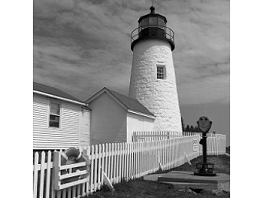
\includegraphics{1} & 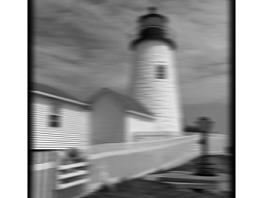
\includegraphics{2} & 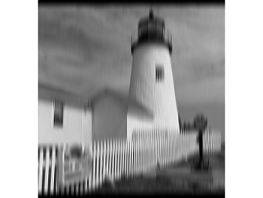
\includegraphics{3} & 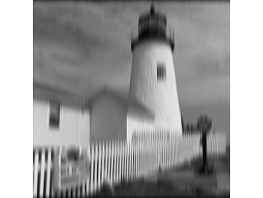
\includegraphics{4}\\
  Original Image & Rows Filtered & Columns Filtered & 2D Filter and Trimmed\\
\end{tabular}
\caption{Low-pass filtering with half-cosine filter showing edge fading artefacts}
\end{centering}
\end{figure}

Symmetric extension is a technique which minimises the edge effects of filtering. The images below have been symmetrically extended and then the low-pass filter has been applied hence edge effects are significantly decreased. It does not matter whether the rows or the columns are filtered first since the filter has unit gain and is linearly separable. If two filtered images are formed, one by doing the rows followed by the columns and the other the reverse, the maximum absolute pixel difference is found to be 0.
\begin{figure}[ht!]
\begin{centering}
\begin{tabular}{c c c c}
  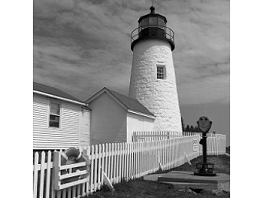
\includegraphics{5} & 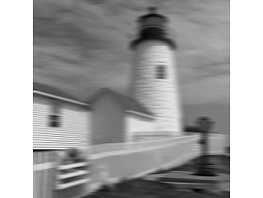
\includegraphics{6} & 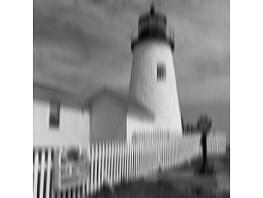
\includegraphics{7} & 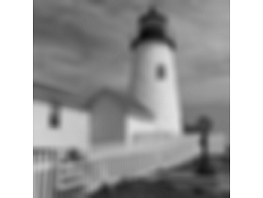
\includegraphics{8}\\
  Original Image & Rows Filtered & Columns Filtered & 2D Filter and Trimmed\\
\end{tabular}
\caption{Low-pass filtering with half-cosine filter and symmetrically extended image}
\end{centering}
\end{figure}

A high pass image filter was found by subtracting the low-pass image from the original. It was found that the energy of the high-pass images ($4.7950\times 10^7$) was significantly smaller than that of the low-pass images ($1.25650\times 10^9$) (Values for 4-layer reconstruction).
\begin{figure}[ht!]
\begin{centering}
\begin{tabular}{c c c}
  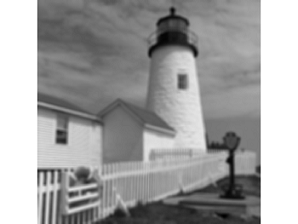
\includegraphics{10} & 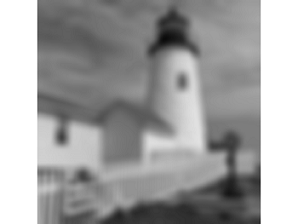
\includegraphics{14} & 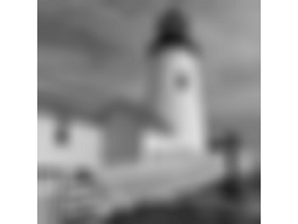
\includegraphics{12}\\
  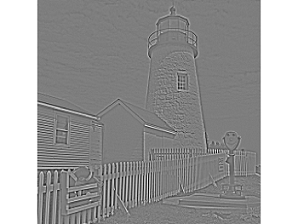
\includegraphics{11} & 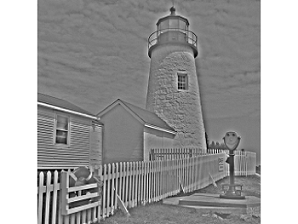
\includegraphics{9} & 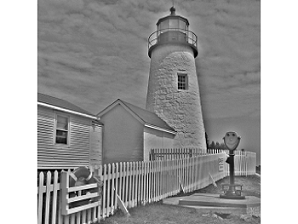
\includegraphics{13}\\
  $len(h) = 5$ & $len(h) = 15$ & $len(h) = 25$\\
\end{tabular}
\caption{Low-pass and high pass filtering with different length half-cosine filters}
\end{centering}
\end{figure}

\section{The Laplacian Pyramid}
A Laplacian Pyramid is a technique which splits the original image up into smaller and smaller pairs of high-pass and low-pass filtered images. The image can then be reconstructed perfectly with the smallest low-pass image and all of the high-pass images. Below is a 4-level Laplacian Pyramid for the lighthouse image.
\begin{figure}[ht!]
\begin{centering}
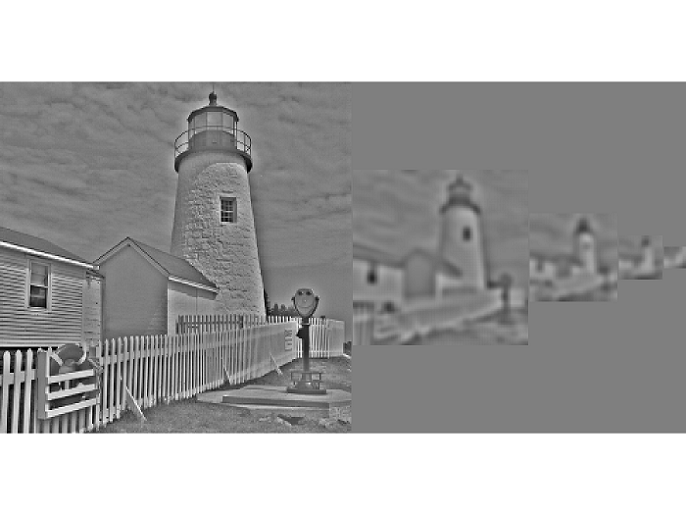
\includegraphics{15}
\caption{4-Layer Laplacian Pyramid for Lighthouse Image}
\end{centering}
\end{figure}
Quantisation allows us to compress the image however it also reduces image quality. The number of bits required to encode X1 and Y0 is $2.15\times 10^5$ compared to $2.28\times 10^5$ bits required to encode X. As the number of layers increases, the number of bits required to encode the image data decreases however reconstructed image quality also decreases. The figure below shows various images which have been encoded with an n-layer Laplacian Pyramid, quantised with a step-size of 17 and reconstructed. The RMS error between the reconstructed and original image is also measured. The image contains some artefacts including the loss of detail in the sky, the block like formation in the building centre and the silhouette effect around the sharp edges of objects.
\newpage
\begin{figure}[ht!]
\begin{centering}
\begin{tabular}{c c c}
  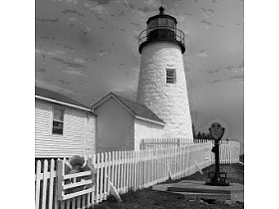
\includegraphics{16} & 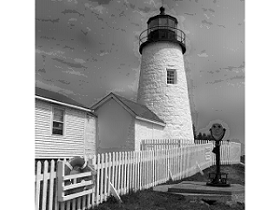
\includegraphics{17} & 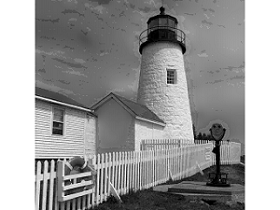
\includegraphics{18}\\
  $n=4$,  $RMS = 5.6189$ & $n=5$, $RMS = 5.9068$ & $n=6$, $RMS = 5.6520$\\
\end{tabular}
\caption{n-Layer Quantised Laplacian Pyramid reconstruction Lighthouse Image}
\end{centering}
\end{figure}

Since image quality is reduced by quantisation, comparing number of bits for different coding schemes is only valid if difference in RMS error of a directly quantised image to that of the reconstructed quantised image and minimised. This is achieved by finding the optimal step size for a given initial step size and pyramid depth. The figure below shows the image directly quantised with a step size of 17. The RMS error was measured to be $4.8612$.
\begin{figure}[ht!]
\begin{centering}
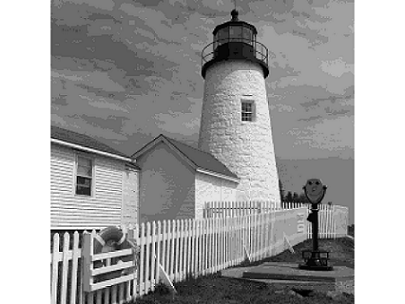
\includegraphics{19}
\caption{4-Layer Laplacian Pyramid for Lighthouse Image}
\end{centering}
\end{figure}\\

The optimal step size when comparing to a direct quantisation with step size 17 was found for different numbers of level Laplacian Pyramids outlined in the table below (Table 1).
\begin{table}[h!]
\begin{centering}
\begin{tabular}{|l|l|}
\hline
Number of Levels & Optimal Step Size \\ \hline
1                & 15.2              \\ \hline
2                & 13.2              \\ \hline
3                & 11.6              \\ \hline
4                & 10.3              \\ \hline
5                & 9.5               \\ \hline
6                & 8.6               \\ \hline
\end{tabular}
\caption{Optimal Step Size for n-Layer Laplacian Pyramid}
\end{centering}
\end{table}\\

\section{Constant Step Size and Equal MSE Criterion}
There are two parameters for the Laplacian Pyramid technique: The number of levels and the quantisation step size. The number of bits required can be minimised in two ways, either using a constant step size or by using an equal MSE criterion. \\

For a constant step size we can optimise over the layer depth of the Laplacian Pyramid in order to produce the scheme which required the least number of bits to encode for the step size which has same RMS error as directly quantising the image.

The MSE criterion can be used to further refine this optimisation by varying the step sizes for each layer according to the impulse response from each layer. In order to perform this optimisation, the MSE ratios of impulse responses had to be found and are shown in Table 2. Also the optimal set of step sizes (which had to correspond to these ratios) also had to be found for each number of levels.
\begin{table}[]
\begin{centering}
\begin{tabular}{|l|l|l|}
\hline
Number of Levels & Optimal Step Size for Y0 & MSE fraction of Y0 \\ \hline
1                & 18.56                    & 1                  \\ \hline
2                & 18.5                     & 0.6667             \\ \hline
3                & 18.1                     & 0.3637             \\ \hline
4                & 18.08                    & 0.1861             \\ \hline
5                & 18.06                    & 0.0936             \\ \hline
6                & 18.06                    & 0.0469             \\ \hline
\end{tabular}
\caption{Optimal Step Size and MSE step size fraction for each layer}
\end{centering}
\end{table}

Finally, the impact of using a more complicated decimation filter was analysed by using a 5-tap filter used in place of the previous 3-tap. Although more complex, it was found that it produced worse compression with lower compression ratio.

The optimal number of layers and associated compression ratios for each scheme are shown in Figure 7 below:

\begin{figure}[ht!]
\begin{centering}
\begin{tabular}{c c}
  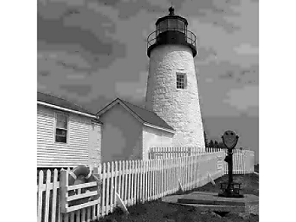
\includegraphics{20} & 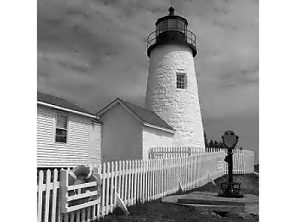
\includegraphics{21} \\
  Constant Step Size & Equal MSE Criterion\\
  $len(h) = 3$ & $len(h) = 3$ \\
  $n = 2$ & $n=4$ \\
  $Bits= 1.6475\times 10^5$ & $Bits= 1.4723\times 10^5$ \\
  $Compression\; Ratio = 1.385$ & $Compression\; Ratio = 1.549$\\
  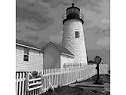
\includegraphics{22} & 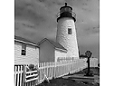
\includegraphics{23}\\
  Constant Step Size & Equal MSE Criterion\\
  $len(h) = 5$ & $len(h) = 5$\\
  $n = 2$ & $n=3$\\
  $Bits= 1.711\times 10^5$ & $Bits= 1.605\times 10^5$\\
  $Compression\; Ratio = 1.333$ & $Compression\; Ratio = 1.421$\\
\end{tabular}
\caption{Optimal Reconstructed Images for Constant Step Size and Equal MSE Criterion}
\end{centering}
\end{figure}
\end{document}							%End of the document.
